\documentclass{beamer}

\usepackage{beamerthemesplit}
\usepackage{verbatim}
\usepackage[normalem]{ulem}

\usepackage{xcolor}

\usepackage{hyperref}

\definecolor{gold}{rgb}{1.,0.84,0.}
\definecolor{brightred}{rgb}{1.,0.4,0.4}
\definecolor{mygray}{RGB}{200,200,200}
\definecolor{lightsteelblue}{RGB}{176,196,222}
\definecolor{lightskyblue}{RGB}{135,206,250}
\definecolor{cadetblue}{RGB}{95,158,160}

\usetheme{default}
\usecolortheme{mule}

\usefonttheme{serif}

%\DeclareGraphicsExtensions{.pdf,.png,.jpg}

\newcommand{\mcal}{\textsc{metacalibration}}
\newcommand{\Mcal}{\textsc{Metacalibration}}

\newcommand{\mcalR}{\mbox{\boldmath $R$}}
\newcommand{\mcalRscalar}{\mbox{$R$}}

\newcommand{\mcalRmean}{\mbox{\boldmath $\langle R \rangle$}}
\newcommand{\mcalRscalarmean}{\mbox{$\langle R \rangle$}}

\newcommand{\mcalRpsf}{$R^{p}$}
\newcommand{\mcalRpsfnoise}{$R^{p}_\eta$}
\newcommand{\mcalRo}{\mbox{\boldmath $R_o$}}
\newcommand{\mcalRnoise}{\mbox{\boldmath $R_\eta$}}

\newcommand{\mcalRmeanalpha}{\mbox{\boldmath $\langle R_\alpha \rangle$}}
\newcommand{\mcalRmeanbeta}{\mbox{\boldmath $\langle R_\beta \rangle$}}

\newcommand{\mcalRg}{\mbox{\boldmath $R_\gamma$}}
\newcommand{\mcalRS}{\mbox{\boldmath $R_S$}}
\newcommand{\mcalRgmean}{\mbox{\boldmath $\langle R_\gamma \rangle$}}
\newcommand{\mcalRSmean}{\mbox{\boldmath $\langle R_S \rangle$}}

\newcommand{\mcalRtwopt}{\mbox{\boldmath $R^{2pt}$}}
\newcommand{\mcalRtwoptmean}{\mbox{\boldmath $\langle R^{2pt} \rangle$}}


\newcommand{\mcalRmodel}{\mbox{\boldmath $R^{model}$}}
\newcommand{\mcalRnoisemodel}{\mbox{\boldmath $R^{model}_\eta$}}


\newcommand{\vecg}{\mbox{\boldmath $\gamma$}}
\newcommand{\vest}{\mbox{\boldmath $e$}}

\newcommand{\snr}{$S/N$}
\newcommand{\snT}{$(S/N)_{\textrm{size}}$}
%\newcommand{\snT}{$\left( \frac{S}{N}\right)_{\textrm{size}}$}
\newcommand{\snflux}{$(S/N)_{\textrm{flux}}$}
%\newcommand{\snflux}{$\left( \frac{S}{N}\right)_{\textrm{flux}}$}

\newcommand{\lensfit}{\texttt{LENSFIT}}
\newcommand{\numba}{\texttt{Numba}}
\newcommand{\python}{\texttt{Python}}
\newcommand{\ngmix}{\texttt{ngmix}}
\newcommand{\ngmixer}{\texttt{ngmixer}}
\newcommand{\shear}{{\bf g}}
\newcommand{\redmapper}{redMaPPer}
\newcommand{\est}{$e$}


\newcommand{\prelim}{{\bf{\it Preliminary}}}

\newcommand{\uberseg}{{\color{lightsteelblue} {\"u}berseg}}
\newcommand{\MOF}{{\color{brightred}MOF}}


\title{Using Coadds for Photometry and Shear}
\author{Erin Sheldon}
\institute{Brookhaven National Laboratory}

% http://texblog.net/latex-archive/plaintex/beamer-footline-frame-number/
% to add the page (frame ) number and not screw up the bottom line
% works for split themes?
\expandafter\def\expandafter\insertshorttitle\expandafter{%
      \insertshorttitle\hfill%
        \insertframenumber\,/\,\inserttotalframenumber}

% suppress navigation bar
\beamertemplatenavigationsymbolsempty
\setbeamertemplate{footline}{}

\begin{document}

\usebackgroundtemplate{%
    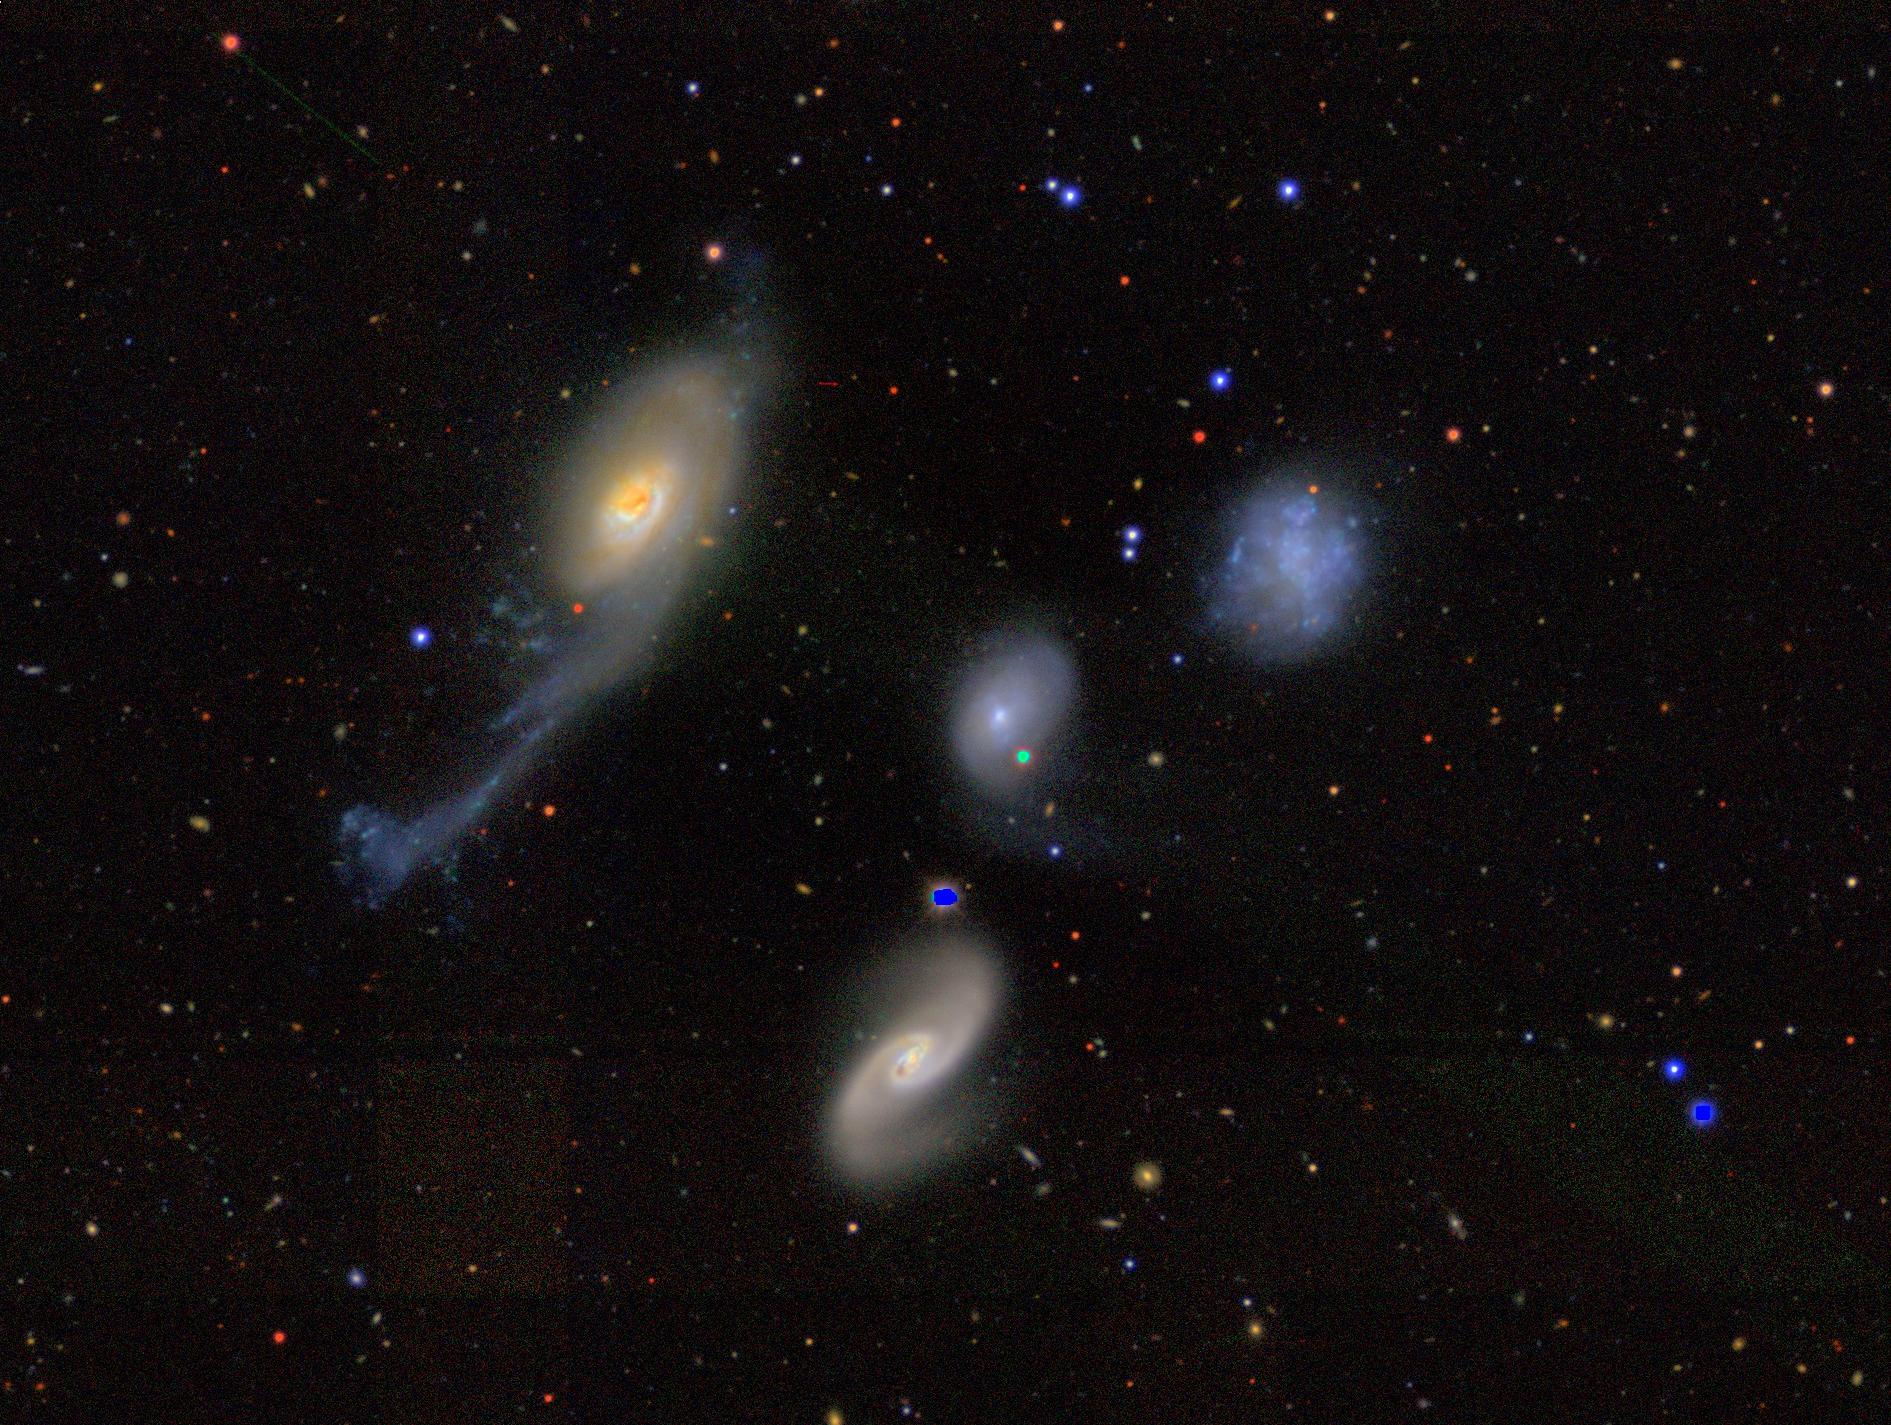
\includegraphics[height=\paperheight]{des0022-4831-four.jpg}
}
\frame
{
}
\setbeamertemplate{background canvas}[vertical shading][bottom=mgray,top=mblack]

\setbeamerfont*{itemize/enumerate body}{size=\Large}
\setbeamerfont*{itemize/enumerate subbody}{parent=itemize/enumerate body}
\setbeamerfont*{itemize/enumerate subsubbody}{parent=itemize/enumerate body}


\frame{\titlepage}




\frame
{
    \frametitle{Outline}

    \begin{itemize}

        \item Introduction to coadds: pros and cons
        \item Mitigating issues with coadds
            \begin{itemize}
                \item Kaiser coadds
                \item Coadd the PSF
                \item Single-object coadds to deal with additional PSF issues
                \item Dealing with correlated noise
            \end{itemize}
        \item Simulation tests
            \begin{itemize}
                \item Noise tests
                \item Shear bias tests
            \end{itemize}
        \item Future Work

    \end{itemize}

}

\frame
{
    \frametitle{Coadds: pros}

    \begin{itemize}

        \item Large data compression:  factor of about 100 for LSST

        \item Corresponding speed up for analysis

        \item Simplifies analysis, don't need to do multi-epoch fitting (but do
            still need multi-band)

    \end{itemize}

}

\frame
{
    \frametitle{Coadds: cons}

    \begin{itemize}

        \item The variance of quantities derived from standard coadds is
            generally higher than a multi-epoch fitting appraoch

        \item The PSF, noise, etc. discontinuous in the coadd at the location
            of edges in original images

        \item The noise is correlated in standard coadds due to interpolation


    \end{itemize}

}

\frame
{
    \frametitle{Example of Increased Variance}
 
    \setbeamerfont*{itemize/enumerate body}{size=\footnotesize}
    \setbeamerfont*{itemize/enumerate subbody}{parent=itemize/enumerate body}
    \setbeamerfont*{itemize/enumerate subsubbody}{parent=itemize/enumerate body}
 
    \begin{itemize}
        \item Template flux, just fitting for an amplitude $A$
        \item We can calculate directly the increased variance
        \item Can also calculate a toy model with Gaussian PSF and object, assume
            Gaussian final image (Sheldon, Armstrong, Huff, et al. in prep)
                \begin{align}
                    \textrm{var}\hat{A}_{\textrm{coadd}} = 
                    \textrm{var}\hat{A}_{\textrm{me}} \left[ 1 + 2 (1-R)^2 \left( \frac{\Delta \sigma_p}{\sigma_p} \right)^2 \right]
                \end{align}

         \item $g$ marks the object and $p$ the PSF
         \item $R = \sigma_g^2/(\sigma_p^2 + \sigma_g^2)$ is 0 for stars, 1 for huge galaxies

         %\item Expect the effect may be smaller for shear because the intrinsic shape noise
         %    is an important part of the variance.

    \end{itemize}


}

\frame
{
    \frametitle{Fluxes: comparison of formula with simulation}
 
        %\newline
        $\Delta \sigma_p/\sigma_p = 0.10$
    \begin{center}
        \colorbox{white}{
            \includegraphics[width=\columnwidth]{{cnoise-fwhm0.90-frac0.10-ntrial100000}.pdf}
        }
        \newline
        (Sheldon, Armstrong, Huff, et al. in prep)
    \end{center}


}

\frame
{
    \frametitle{Mitigating increased variance: Kaiser Coadds}

    \begin{itemize}

        \item For LSST, we expect a very minor increase in variance $(< 1\%)$.

        \item For surveys with large seeing variation, we might care more.

        \item Kaiser derived a more optimal coadd for which there should be no
            increase in variance

        \item However we use in DES and LSST we currently use standard coadds

        \item From here on all the tests I show will be on standard coadds

    \end{itemize}

}



\frame
{
    \frametitle{Mitigating PSF issues: single-object coadds}

    \begin{itemize}

        \item Overcome some discontinuities by coadding the PSF reconstructions
            also (e.g. Annis et al. SDSS coadd)

        \item However if an object crosses an image boundary, the PSF will still not be correct

        \item Solution is single-object coadds: make a coadd for each object
            separately, only including epochs where the object does not hit an
            edge (I heard the idea first from Jim Bosch)


    \end{itemize}

}

\frame
{
    \frametitle{Mitigating correlated noise issues}

    \setbeamerfont*{itemize/enumerate body}{size=\normalsize}
    \setbeamerfont*{itemize/enumerate subbody}{parent=itemize/enumerate body}
    \setbeamerfont*{itemize/enumerate subsubbody}{parent=itemize/enumerate body}
 
    \begin{itemize}

        \item Not a big problem for fluxes, but causes a bias for shear measurement

        \item One can whiten the noise, but it can result in a significant increase in noise

        \item (Kaiser claims no loss of information if done correctly, but I don't understand this yet)

        \item Alternatively: determine the covariance and use it in analyses
            \begin{itemize}
                \item Run noise images through the coadd process also
                \item Feed this image into \mcal
                \item Measure a covariance matrix and use it in BFD (moments only taken once, so this is feasible)
            \end{itemize}


    \end{itemize}

}

\frame
{
    \frametitle{Simulation Tests}

 
    \begin{itemize}

        \item Tested both realistic size and flux distribution, as well as
            fixed size and flux (to isolate any increase in noise).

        \item DES-like seeing distribution.

        \item Ran with typical DES WCS variations
        \item Also ran tests with random rotations like in LSST.

        \item Ran in full multi-epoch mode and coadd mode.

        \item Coadd code by Armstrong \& Sheldon.  Simulation and \mcal\ code
            Sheldon.  BFD code Bob Armstrong.

    \end{itemize}

}


\frame
{
    \frametitle{Increased shear variance}

    \setbeamerfont*{itemize/enumerate body}{size=\normalsize}
    \setbeamerfont*{itemize/enumerate subbody}{parent=itemize/enumerate body}
    \setbeamerfont*{itemize/enumerate subsubbody}{parent=itemize/enumerate body}
 
    \begin{itemize}

        \item Fixed size and flux to test only variation in noise: due to correlated
            noise, quantities used for selection, such as S/N are different for multi-epoch
            and coadd measurements.
            
        \item DES-like
            seeing and PSF ellipticity distribution.

        \item For \mcal\ and BFD we see little increase in the noise
            \begin{itemize}

                \item \mcal\ for the smallest galaxies we would use $(T/T_{\textrm{PSF}} = 0.5)$ and typical $S/N = 15$
                    the noise in the recovered shear increases by 
                    \begin{align}
                    (0.65 \pm 0.02) \%
                    \end{align}

                \item BFD, B. Armstrong reported noise of 0.0007 for both (need more sig. figures)

            \end{itemize}

    \end{itemize}

}

\frame
{
    \frametitle{Increased shear bias}

    \setbeamerfont*{itemize/enumerate body}{size=\normalsize}
    \setbeamerfont*{itemize/enumerate subbody}{parent=itemize/enumerate body}
    \setbeamerfont*{itemize/enumerate subsubbody}{parent=itemize/enumerate body}
 
    \begin{itemize}

        \item Realistic size and galaxy flux distribution.  DES-like seeing and
            PSF ellipticity distribution.


        \item For \mcal\ and BFD we detect no increase in bias
        \item \mcal 
            \begin{align}
            m = (0.56 \pm 0.36) \times 10^{-3}
            \end{align}
            (expect $\sim 0.25 \times 10^{-3}$ due to breakdown of weak shear approx.)

        \item BFD (B. Armstrong)
            \begin{align}
                m = (1.2 \pm 0.7) \times 10^{-3}
            \end{align}



    \end{itemize}

}

\frame
{
    \frametitle{Future Work}

    \setbeamerfont*{itemize/enumerate body}{size=\normalsize}
    \setbeamerfont*{itemize/enumerate subbody}{parent=itemize/enumerate body}
    \setbeamerfont*{itemize/enumerate subsubbody}{parent=itemize/enumerate body}
 
 
    \begin{itemize}

        \item In DES edges are important due to the low number of epochs
            ($\sim10$).

        \item We need to create a code for the single-object coadds and
            corresponding PSF coaddition.  May be able to work this into the
            MEDS maker.  Need to run noise images through as well for
            correlated noise.

        \item For LSST epochs will be rotated: coadds need to be done on the
            full images, or very large initial postage stamps,  to avoid
            artifacts in the ``corners''.

        \item However, for LSST edges are less of a problem due to the large
            number of epochs ($\sim 100$).  It would be good to test in
            simulations if we need the single-object coadds at all.

    \end{itemize}

}


\end{document}
